\section{Radioactive decay analogue}
\label{decay}

%IA practical lab

In this experiment, you will use an analogue of radioactive decay to learn more about random errors in measurement, and to produce a decay curve for a small number of `radioactive' particles.  The only apparatus you will need are a number of cubes, each with one face identified.

\begin{center}
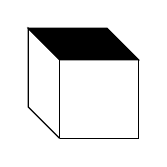
\begin{tikzpicture}
\draw (0,0)--(1,0)--(1,1)--(0,1)--(0,0);
\draw (0,0)--(-0.4,0.4)--(-0.4,1.4)--(0,1);
\draw[fill] (0,1)--(-0.4,1.4)--(0.6,1.4)--(1,1)--(0,1);
\end{tikzpicture}
\end{center}

Because radioactive decay is a randomly activated process, the rolling of cubic dice is an appropriate way to study it.  Measurement of the rate of radioactive decay is subject (like any other measurement in physics) to random fluctuations, i.e.\ repeated measurements of the number of nuclei decaying in a given period of time will not all be equal.  We aim to study the distribution of these measurements in this experiment.

{\bf Unless otherwise indicated, you and your partner should take separate sets of measurements, and do the graphical work and calculations independently.}  You should however work together in making the observations and compare your results.  This will allow you to check for mistakes in your work.

\subsection{A set of readings: mean and standard deviation}

Take 50 of the small cubes, which represent radioactive nuclei.  You need to shake them all up and let them fall onto the desk.  All of the cubes which have landed with the black face uppermost are those which have `decayed' in the time interval of the experiment.  Firstly, you need to obtain a set of 10 measurements of the number of nuclei out of 50 which decay in one timestep (start with 50 each time).\\

\noindent\begin{tabular}{|l|p{0.9cm}|p{0.9cm}|p{0.9cm}|p{0.9cm}|p{0.9cm}|p{0.9cm}|p{0.9cm}|p{0.9cm}|p{0.9cm}|p{0.9cm}|}
\hline
{\bf Measurement} & 1 & 2 & 3 & 4 & 5&6&7&8&9&10\\
\hline
{\bf Decays} &&&&&&&&&&\\
\hline
\end{tabular}

\begin{questions}
\question What is the probability of 1 nuclei decaying in 1 timestep? \answerline

\question How many nuclei do you expect to decay out of 50 in 1 timestep? \answerline

The mean (or average) $\overline{x}$ is normally the best estimate of the true value of a measured quantity, being at the centre of the distribution of reading values. \question Calculate the mean of your 10 measurements: \answerline

We also need a measure of the spread of the measurements.  Conventionally, this is $\sigma$, the {\bf standard deviation} or `sigma'.  You can quickly estimate a value for $\sigma$ using the `range method'\footnote{The range method is good for $n$ up to about 12.}, i.e. if $r$ is the range of a set of $n$ readings (the difference between the largest and smallest values), then an \emph{estimate} of $\sigma$ is given by
\[\sigma=\frac{r}{\sqrt{n}}.\]
\question Estimate the standard deviation of your 10 measurements. \answerline

\subsection{Distribution of means}

One way to correct for the effects of random fluctuations is to find the mean of repeated measurements.  Theory suggests the following formula for $\sigma_{m}$, the standard deviation of the mean of $n$ measurements,
\[\sigma_{m}=\frac{\sigma}{\sqrt{n}}.\]

\question Calculate $\sigma_{m}$ for your mean. \answerline

\question Look at your partners' results and mean.  Do your means agree with the equation above for the case $n=10$?  Make a short comment below.

\fillwithlines{3cm}

\subsection{Presenting the final answer}

The correct, conventional way to present the result of a repeated measurement is as follows:
\[\text{result}=\overline{x}\pm\sigma_{m}.\]
In graphical work, error bars normally run from $\overline{x}-\sigma_{m}$ to $\overline{x}+\sigma_{m}$\\
e.g. $R=4.625\pm 0.007~\Omega$.

The error in a measurement is usually given to one significant figure (sometimes two significant figures if the numerical value starts with a 1), and a result and its error should always be given to the same number of decimal places.

\question Give the result of your set of 10 measurements in the format above. \answerline

\question Give the most accurate result you can (use your partner's results too) in the same format. Show any working. \fillwithlines{2cm}

\subsection{Radioactive decay}

You are now going to simulate radioactive decay, by removing those dice which `decay' at each turn, and re-rolling the remaining dice for each timestep.  Record your own results in the table below, and then add your results to those of your partner to give a total in the column for this purpose.

\begin{tabular}{|c|c|c|c|c|}
\hline
Time & Number remaining & Pooled results & Mean\footnote{Divide your pooled results by the number in your group to get the average result.} & Estimated spread\\
$t$ & $x$ & $\sum{x}$ & $\overline x$ & $\sigma_{m}$\\
\hline
0 & 50 & & 50 &\\
\hline
1 & &&&\\
\hline
2 & &&&\\
\hline
3 & &&&\\
\hline
4 & &&&\\
\hline
5 & &&&\\
\hline
6 & &&&\\
\hline
7 & &&&\\
\hline
8 & &&&\\
\hline
9 & &&&\\
\hline
10 & &&&\\
\hline
11 & &&&\\
\hline
12 & &&&\\
\hline
\end{tabular}\\

\question Now plot a graph of $\overline{x}$ on the vertical axis against $t$ on the horizontal axis, and draw a trend line.  Your results ought to be quite similar to those expected from radioactive decay.  The trend should be the same, and there is also some randomness.

\question Comment on your results.  It the trend as you expect?  How close are the points to the line of best fit? \fillwithlines{3cm}

A close match between the results from this model and the results from real radioactivity would strongly suggest that individual radioactive atoms decaying at random with a fixed probability in any given time interval.  This experiment also helps to `explain' the downward trend of the decay curve: only dice that are left can `decay', and as there are fewer of them each time, fewer will decay.

\question How does the pooling of results make your $\overline{x}$ more accurate than your $x$? \fillwithlines{3cm}

\question This activity raises the interesting question about how long a radioactive source will last.  What happens to the last `atom'?  Comment below.  \fillwithlines{2cm}
\end{questions}
